\begin{figure}[t]
  \centering
  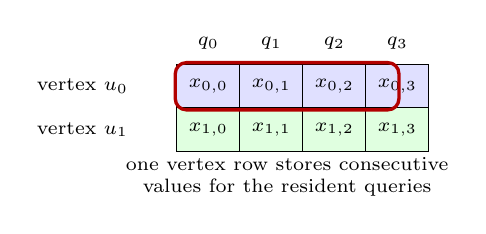
\begin{tikzpicture}[
      font=\scriptsize,
      cell/.style={draw, minimum width=8mm, minimum height=5.5mm, inner sep=0pt},
      lab/.style={align=right}
    ]
    \node[lab] at (-1.2,0) {vertex $u_0$};
    \node[lab] at (-1.2,-0.55) {vertex $u_1$};
    \foreach \x/\q in {0/0,1/1,2/2,3/3} {
      \node at (0.4+0.8*\x,0.55) {$q_{\q}$};
      \node[cell, fill=blue!12] at (0.4+0.8*\x,0) {$x_{0,\q}$};
      \node[cell, fill=green!12] at (0.4+0.8*\x,-0.55) {$x_{1,\q}$};
    }
    \draw[very thick, red!70!black, rounded corners] (-0.02,-0.3) rectangle (2.82,0.3);
    \node[align=center] at (1.4,-1.15) {one vertex row stores consecutive\\values for the resident queries};
  \end{tikzpicture}
  \caption{Vertex-major $V\!\times\!Q$ state layout used by \coalescedgather.  Holding the graph vertex fixed while varying the query identifier turns the query dimension into a contiguous access sequence.}
  \Description{A two-row value matrix with vertices as rows and resident queries as contiguous columns. A highlighted row contains all query values for one graph vertex.}
  \label{fig:layout}
\end{figure}
